\documentclass{article}
\usepackage{tikz}
\usepackage{natbib}
\title{Problem set on hierarchical models and ODEs}
\date{}
\usepackage{caption}
\captionsetup{font=footnotesize}
\usepackage[utf8]{inputenc}
\usepackage{amsmath}
\usepackage{multimedia}
\usepackage{animate}
\usepackage{graphics}
\usepackage{graphicx}
\usepackage[makeroom]{cancel}
\newtheorem{problem}{Problem}[section]
\usepackage{bbm}
\author{Ben Lambert}
\usepackage{listings}% Encoding: UTF-8

\usepackage{minted}

\begin{document}
\maketitle

\section{A meta-analysis of beta blocker trials}
Table \ref{tab:observedData} shows the results of some of the 22 trials included in a meta-analysis of clinical trial data on the effect of beta-blockers on reducing the risk of myocardial infarction \citep{carlin1992meta}. The file ``prob5\_betaBlocker.csv'' contains the full dataset.

The aim of this meta-analysis is to determine a robust estimate of the effect of beta-blockers by pooling information from a range of previous studies.

\begin{table}[htbp]
	\centering
	\caption{The data from the original study.}
	\begin{tabular}{ccc}
		& \multicolumn{2}{c}{\textbf{Mortality: deaths/total}} \\
		\textbf{Study} & \textbf{Treated} & \textbf{Control} \\
		1     & 3/38  & 3/39 \\
		2     & 7/114 & 14/116 \\
		3     & 5/69  & 11/93 \\
		4     & 102/1533 & 127/1520 \\
		...    &       &  \\
		20    & 32/209 & 40/218 \\
		21    & 27/391 & 43/364 \\
		22    & 22/680 & 39/647 \\
	\end{tabular}%
	\label{tab:observedData}%
\end{table}%

\begin{problem}
	Start by assuming that the numbers of deaths in the control ($r^c_i$) and treated ($r^t_i$) groups for each trial are given by binomial distributions of the form:
	\begin{align}
	r^c_i &\sim \text{binomial}(p^c_i,n^c_i)\\
	r^t_i &\sim \text{binomial}(p^t_i,n^t_i)
	\end{align}
	
	where $(n^t_i,n^c_i)$ are the numbers of individuals in the treatment and control datasets respectively. Further assume that the probabilities of mortality in the treatment and control datasets are given by:
	
	\begin{align}
	logit(p^c_i) &= \mu_i\\
	logit(p^t_i) &= \mu_i + \delta_i \\
	\end{align}
	
	where $logit(x) = log\left(\frac{x}{1-x}\right)$, and we expect $\delta_i<0$ if the beta-blockers have the desired effect.  We assume the following diffuse priors for the parameters
	
	\begin{align}
	\mu_i&\sim N(0,10)\\
	\delta_i &\sim N(0,10)\\
	\end{align}
	
	Estimate the posteriors for $\delta_i$ for the above model using Stan, or otherwise. Note: that for this model there is no inter-dependence between the studies. (Hint: use the Stan function ``binomial\_logit''.)
\end{problem}

The code to estimate this model is given by:

\begin{minted}{stan}
data {
  int<lower=0> N; 
  int<lower=0> nt[N]; 
  int<lower=0> rt[N]; 
  int<lower=0> nc[N]; 
  int<lower=0> rc[N]; 
} 
parameters {
  vector[N] mu;
  vector[N] delta;
} 
model {
  rt ~ binomial_logit(nt, mu + delta);
  rc ~ binomial_logit(nc, mu);
  delta  ~ normal(0,10); 
  mu ~ normal(0, 10);
}
\end{minted}

The posteriors for $\delta_i$ in this model are fairly wide and contain non-zero densities at zero (figure \ref{fig:prob5_delta}).

\begin{figure}[ht]
	\centerline{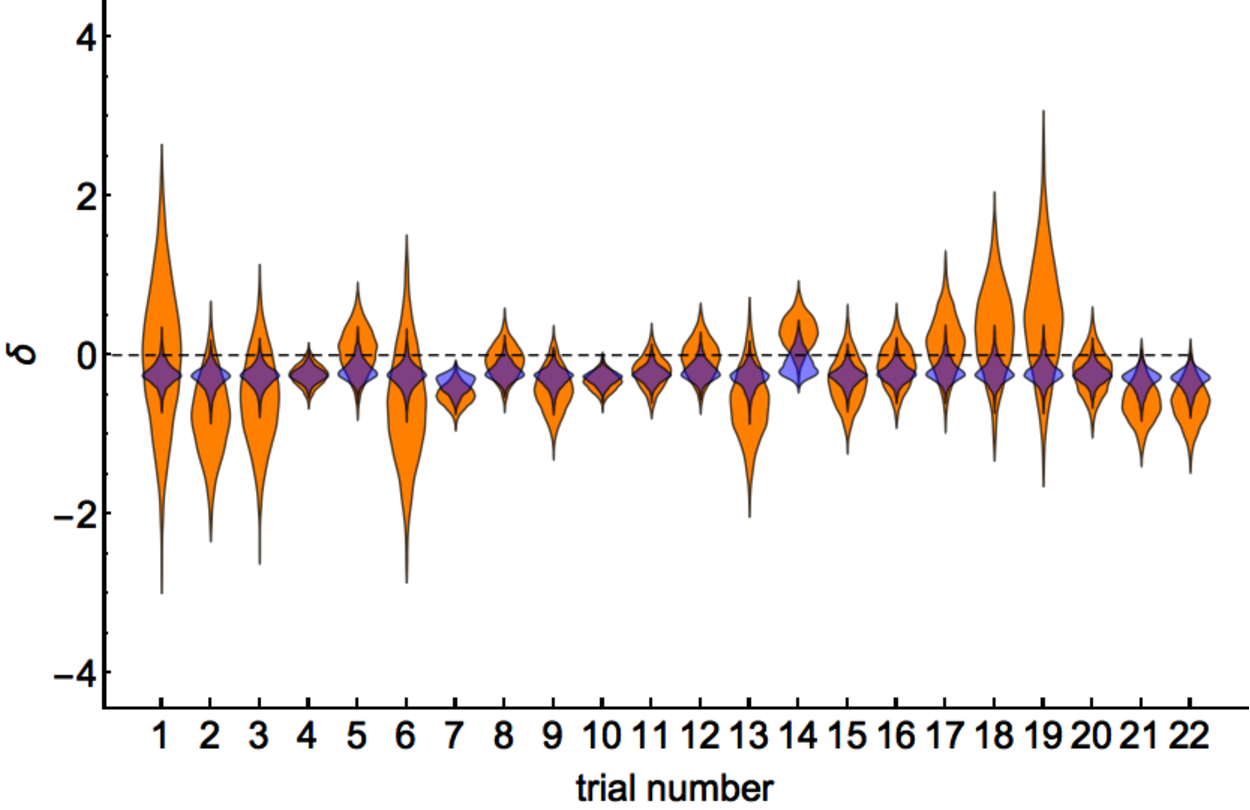
\includegraphics[width=1.5\textwidth]{figures/prob5_betaBlockerDelta.pdf}}
	\caption{The posterior estimates of $\delta_i$ for the fully-heterogeneous (orange) and hierarchical (blue) models.}\label{fig:prob5_delta}
\end{figure}

\begin{problem}
	An alternative framework is a hierarchical model where we assume there to be a common over-arching distribution, across trials such that $\delta_i\sim N(d,\sigma)$. By assuming the following priors on these parameters estimate this model:
	\begin{align}
	d&\sim N(0,10)\\
	\sigma &\sim cauchy(0,2.5) \text{, for }\sigma\geq 0
	\end{align}
	
	Estimate the posteriors for $\delta_i$ using Stan. How do these estimates compare to the non-hierarchical model?
\end{problem}

The code for this problem is shown below:

\begin{minted}{stan}
data {
  int<lower=0> N; 
  int<lower=0> nt[N]; 
  int<lower=0> rt[N]; 
  int<lower=0> nc[N]; 
  int<lower=0> rc[N]; 
} 
parameters {
  real d;
  real<lower=0> sigma; 
  vector[N] mu;
  vector[N] delta;
} 
model {
  rt ~ binomial_logit(nt, mu + delta);
  rc ~ binomial_logit(nc, mu);
  delta  ~ normal(d, sigma); 
  mu ~ normal(0, 10);
  d ~ normal(0, 10); 
  sigma ~ cauchy(0, 2.5);
}
\end{minted}

When I used the above code I ran into a few divergent iterations - this should \textbf{not} be ignored, and is best handled by increasing adapt\_delta=0.95 when calling Stan. This should help the sampler avoid taking too large steps, and diverging in areas of high posterior curvature.  The problematic regions of parameter space here are due to the correlation in estimates between $d$ and the various $\delta_i$; this is unsurprising, each trial only has a relatively small data sample. As such, it is difficult to disentangle the specific individual study effects from the overall effect $d$.

The hierarchical estimates of the effect of the drug are much more concentrated (figure \ref{fig:prob5_delta}) - by pooling data across all studies we are better able to precisely estimate the effect of the drug. These indicate that the beta-blockers appear to act as desired - decreasing the probability of mortality. 

\begin{problem}
	Using the hierarchical model estimate the cross-study effect of the beta-blockers. (Hint: use the ``generated quantities'' code block.)
\end{problem}

The code for to sample an overall $\delta$ is given below:
\begin{minted}{stan}
generated quantities {
  real delta_overall;
  delta_new = normal_rng(d, sigma);
}
\end{minted}

Overall we estimate a negative value for $\delta$ (figure \ref{fig:prob5_deltaOverall}). Whilst the posterior does overlap zero, we are fairly confident in concluding that $\delta<0$.

\begin{figure}[ht]
	\centerline{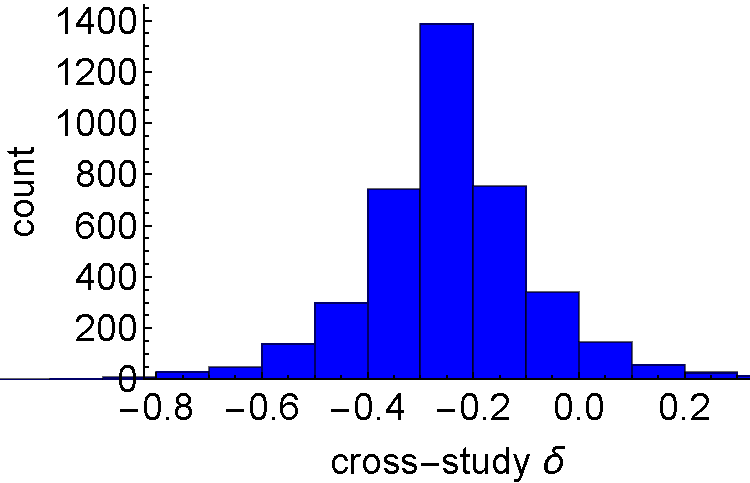
\includegraphics[width=1\textwidth]{figures/prob5_crossStudyDelta.pdf}}
	\caption{The posterior estimate of $\delta$  across all trials for the hierarchical model.}\label{fig:prob5_deltaOverall}
\end{figure}

\begin{problem}
	For an out of sample trial suppose we know that $\mu_i = -2.5$. Using the cross-study estimates for $\delta$ estimate the reduction in probability for a patient taking the beta-blockers.
\end{problem}

This is done by using the inverse-logit transformation (the logistic sigmoid). Essentially you want to evaluate logistic-sigmoid(-2.5) and compare it with logistic-sigmoid(-2.5-delta), across all the samples in your model. This results in a posterior distribution that is peaked at about 0.015 (figure \ref{fig:prob5_risk}); indicating about a 1.5\% reduction in mortality risk for those patients taking beta-blockers.

\begin{figure}[ht]
	\centerline{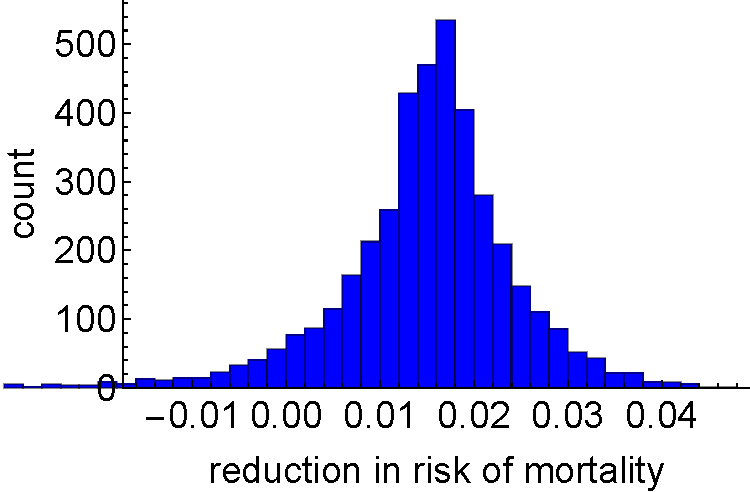
\includegraphics[width=1\textwidth]{figures/prob5_crossStudyRiskReduction.pdf}}
	\caption{The posterior estimates of the reduction in mortality risk associated with taking a beta-blocker when $\mu=-2.5$.}\label{fig:prob5_risk}
\end{figure}

\begin{problem}
	Estimate a model with a single, constant value of $\delta$ and $\mu$ across all trials. Graph the posterior for $\delta$, and compare it with the cross-study hierarchical model estimate.
\end{problem}

The non-hierarchical model gives us a false confidence in our estimates of $\delta$, by assuming that the data from the individual studies are equivalent (exchangeable). This means that the estimate of $\delta$ obtained is more concentrated than for the hierarchical model (figure \ref{fig:prob5_deltaComparison}).

\begin{figure}[ht]
	\centerline{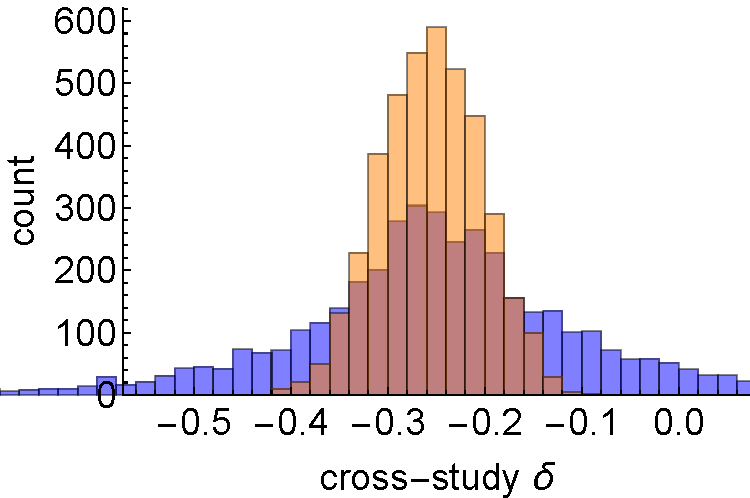
\includegraphics[width=1\textwidth]{figures/prob5_deltaComparison.pdf}}
	\caption{The posterior estimates of cross-study $\delta$ for the hierarchical (blue) and homogeneous (orange) models.}\label{fig:prob5_deltaComparison}
\end{figure}

\begin{problem}
	Carry out appropriate posterior predictive checks on the homogeneous and hierarchical models, and hence conclude the preferred modelling choice.
\end{problem}

One check to do here is to generate posterior predictive data sets of the same shape as the real data, and for each trial record whether the simulated value is greater than the actual. This can be done fairly easily using the ``generated quantities'' block (shown here for the homogeneous model):

\begin{minted}{stan}
generated quantities {
  int<lower=0> simTreatMort[N];
  int<lower=0> simContrMort[N];
  int indicatorTreat[N];
  int indicatorContr[N];
  for (i in 1:N) {
    simTreatMort[i] = binomial_rng(nt[i], inv_logit(mu + delta));
    simContrMort[i] = binomial_rng(nc[i], inv_logit(mu));
    indicatorTreat[i] = (simTreatMort[i] > rt[i]);
    indicatorContr[i] = (simContrMort[i] > rc[i]);
  }
}
\end{minted}

Doing this for both models we find that there are a range of Bayesian p values near 0 or 1 for the homogeneous model, whereas this is not the case for the hierarchical model (figure \ref{fig:prob5_betaBlockerPPCs}.) Intuitively - by assuming that there was no difference between the data from each study - the homogeneous coefficient model is unable to replicate the degree of variation we see in the real data. We therefore prefer the hierarchical model.

\begin{figure}[ht]
	\centerline{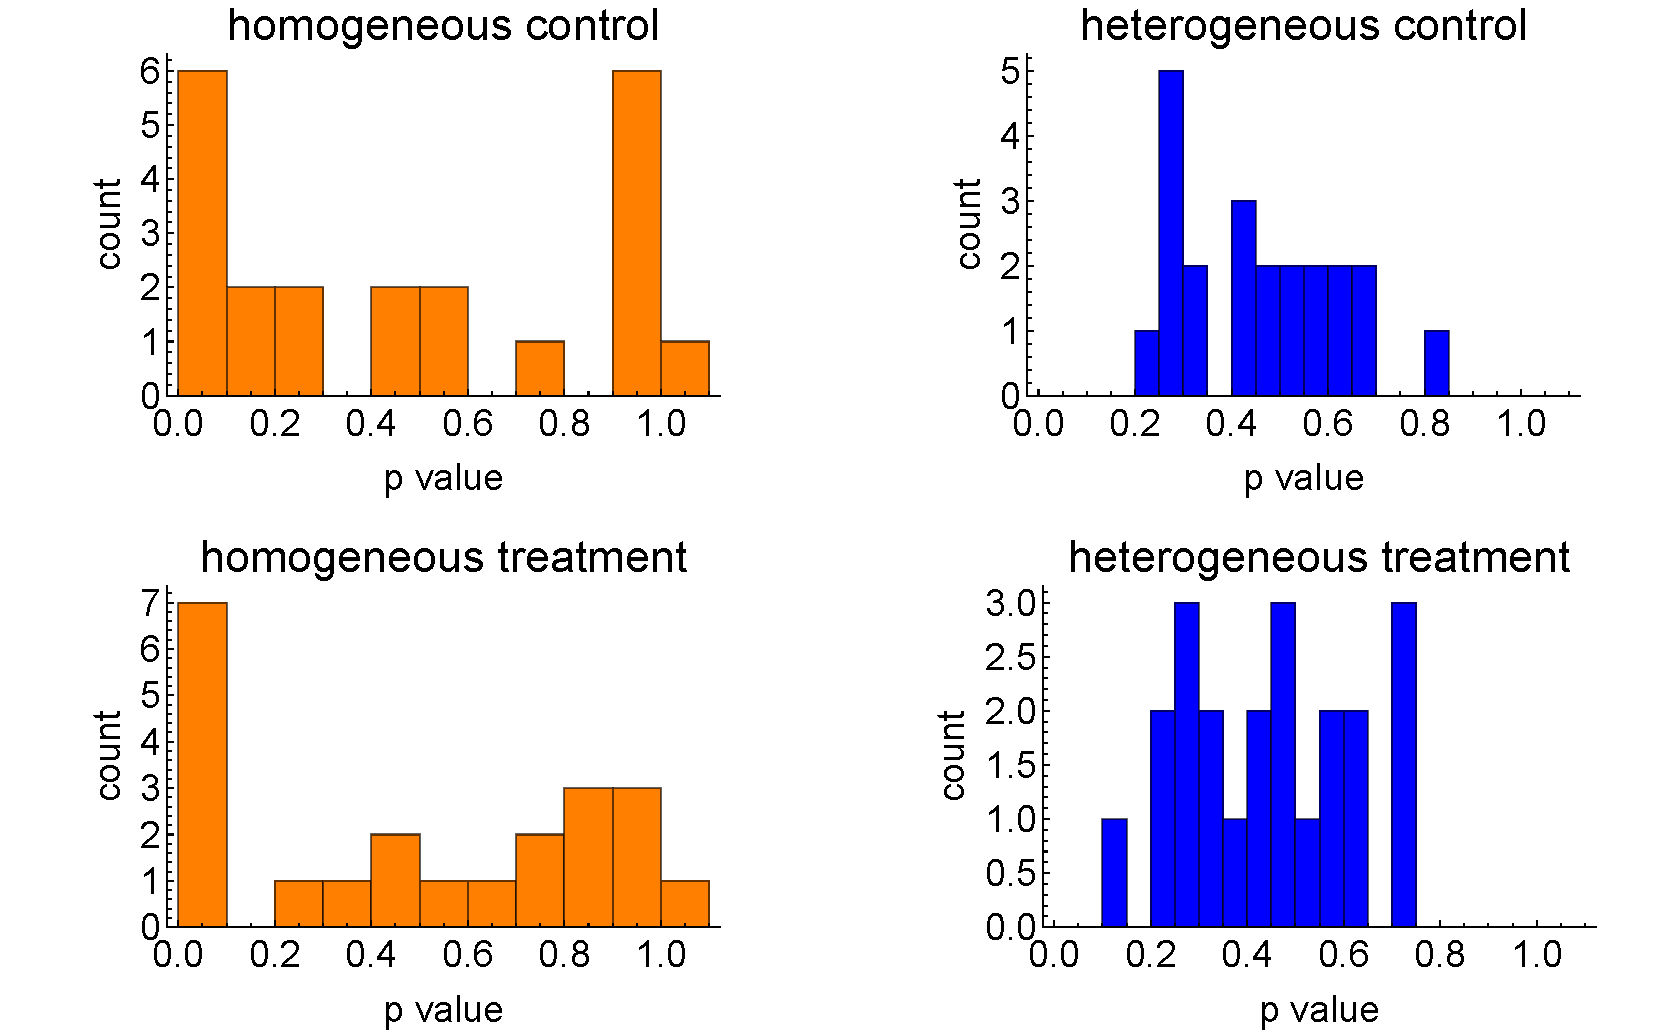
\includegraphics[width=1.5\textwidth]{figures/prob5_betaBlockersPPCs.pdf}}
	\caption{The distribution of Bayesian p values measuring whether the posterior predictive data exceeds the actual across each of the 22 trials for the homogeneous (orange) and hierarchical (blue) models.}\label{fig:prob5_betaBlockerPPCs}
\end{figure}

\section{I can't get no sleep}
These data are from a study described in Belenky et al. (2003) \cite{belenky2003patterns} that measured the effect of sleep deprivation on cognitive performance. There were 18 subjects chosen from a population of interest (lorry drivers) who were restricted to 3 hours of sleep during the trial. On each day of the experiment their reaction time to a visual stimulus was measured. The data for this example are contained within ``prob5\_sleepstudy.csv'', and contains three variables: Reaction, Days and Subject ID which measure the reaction time of a given subject on a particular day.

A simple model that explains the variation in reaction times is a linear regression model of the form:

\begin{equation}
R(t) \sim N(\alpha + \beta t,\sigma)
\end{equation}

where $R(t)$ is the reaction time on day $t$ of the experiment across all observations. 

\begin{problem}
	Assuming normal(0,250) priors on both $\alpha$ and $\beta$ code up the above model in Stan. Use it to generate 1000 samples per chain, across 4 chains. Has the sampling algorithm converged?
\end{problem}

\begin{minted}{stan}
data {
  int N; // number of observations
  matrix[N,2] X; // ones + days of sleep deprivation
  vector[N] R; // reaction times
} 
parameters {
  vector[2] gamma;
  real<lower=0> sigma;
} 
model {
  // likelihood
  R ~ normal(X * gamma, sigma);
  gamma ~ normal(0,250);
}
\end{minted}

After the requisite number of iterates the value for $\hat{R}< 1.1$, meaning it appears that the sampling distribution has converged.

\begin{problem}
	Plot the posterior samples for $\alpha$ and $\beta$. What is the relationship between the two variables, and why?
\end{problem}

There is a strong negative correlation between the estimates of these two variables. This is because to generate a line going through the centre of the dataset, if the intercept increases, the gradient must decrease.

\begin{problem}
	By using the ``generated quantities'' code block or otherwise generate samples from the posterior predictive distribution. By overlaying the real time series for each individual on a graph of the posterior predictive comment on the fit of the model to data.
\end{problem}

The posterior predictive distribution - whilst being a reasonable fit to the data for the anonymous data - is not able to fit well the data at the individual level (figure \ref{fig:lec6_sleepPPC2}). 

\begin{figure}[ht]
	\centerline{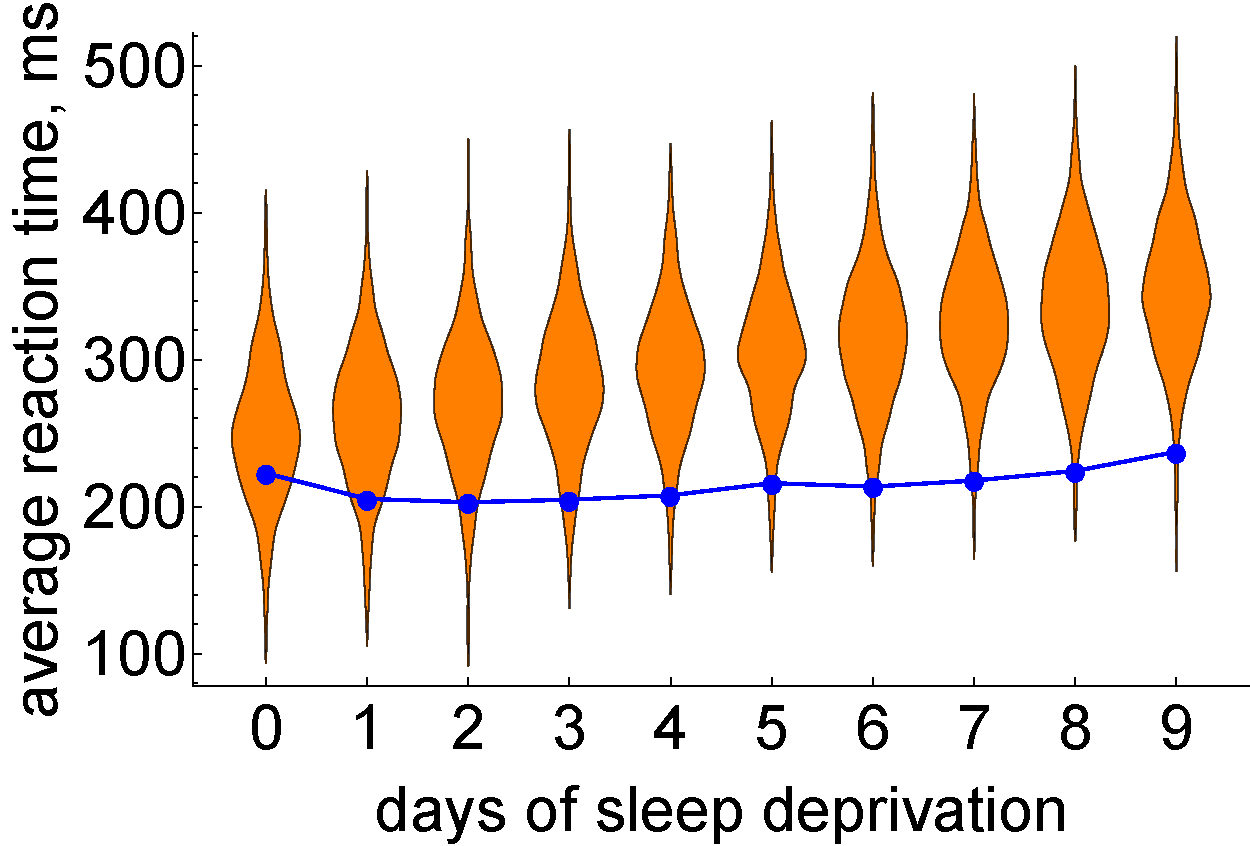
\includegraphics[width=1.25\textwidth]{figures/lec6_sleepPPC2.pdf}}
	\caption{The posterior predictive distribution (orange) and the data for one individual in the sleep study (blue) using the ``homogeneous coefficients'' model.}\label{fig:lec6_sleepPPC2}
\end{figure}

\begin{problem}
	Fit a model with separate $(\alpha,\beta)$ for each individual in the dataset. Use separate and independent normal(0,250) priors for the parameters. Again use 1000 samples per chain over 4 chains.
\end{problem}

This is best done by creating an index of 1 to 18; corresponding to individual subject ID. The model can then be coded up as below:

\begin{minted}{stan}
data {
  int N; // Number of observations
  vector[N] t; // days of sleep deprivation
  vector[N] R; // The reaction times of individuals in the study
  int subject[N]; // Subject ID
}
parameters {
  real alpha[18];
  real beta[18];
  real<lower=0> sigma;
} 
model {
  for (i in 1:N){
    R[i] ~ normal(alpha[subject[i]] + beta[subject[i]] * t[i], sigma);
  }
  alpha ~ normal(0,250);
  beta ~ normal(0,250);
  sigma ~ normal(0,50);
}
\end{minted}

\begin{problem}
	Compute the posterior mean estimates of the $\beta$ parameters for the new ``heterogeneous-parameters'' model. How do these compare to the single $\beta$ estimate obtained for the homogeneous model?
\end{problem}

The homogeneous estimate is about 10.4, with the heterogeneous estimates ranging from -2.8 (for subject 9) to 21.9 (for subject 1). Overall the heterogeneous estimates should have a mean that is roughly similar to the single estimate (it's not exactly so).

\begin{problem}
	Using the ``generated quantities'' code block, or otherwise, generate samples from the posterior predictive distribution. By comparing individual subject data to the posterior predictive samples, comment on the fit of the new model.
\end{problem}

The posterior predictive distribution can be generated in similar fashion to previously, but using the individual subject IDs as an array index.
\begin{minted}{stan}
generated quantities {
  vector[N] R_simulated; // Store post-pred samples
  for (i in 1:N){
    R_simulated[i] =normal_rng(alpha[subject[i]] + beta[subject[i]] * t[i], sigma);
  }
}
\end{minted}

The heterogeneous coefficients model is able to fit the data much more effectively at the individual data (figure \ref{fig:lec6_sleepPPCHetero}). This is unsurprising - essentially we may be guilty of overfitting the model to the data.

\begin{figure}[ht]
	\centerline{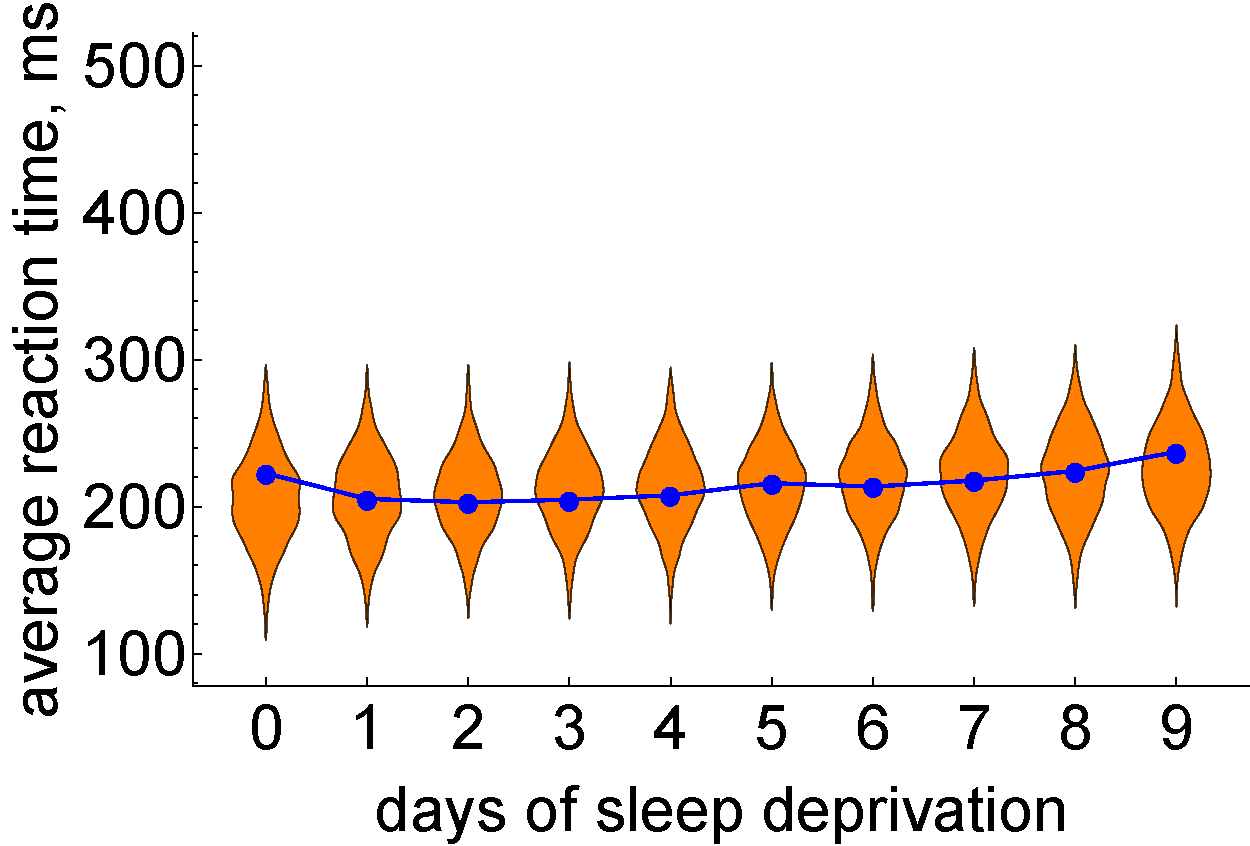
\includegraphics[width=1.25\textwidth]{figures/lec6_sleepPPCHeterogeneous1.pdf}}
	\caption{The posterior predictive distribution (orange) and the data for one individual in the sleep study (blue) using the ``heterogeneous coefficients'' model.}\label{fig:lec6_sleepPPCHetero}
\end{figure}

\begin{problem}
	Partition the data into two subsets: a training set (of subjects 1-17) and a testing set (of subject 18 only). By fitting both models - the heterogeneous and homogeneous coefficients models - on the training sets, compare the performance of each model on predicting the test set data.
\end{problem}
To do this I create two new data variables that hold only the data for the 18th subject. I then change the original data so that it only holds data for subjects 1-17. Of course these manipulations could be handled directly in the Stan code itself, but I prefer to do this outside. The code for the heterogeneous model is shown below:

\begin{minted}{stan}
data {
  int N; // Number of observations in training set
  vector[N] t; // days of sleep deprivation in training set
  vector[N] R; // The reaction times of individuals in the training set
  int subject[N];
  int N2; // Number of data points in the test set
  vector[N2] t2; // Time obs in test set
}
parameters {
  real alpha;
  real beta;
  real<lower=0> sigma;
} 
model {
  for (i in 1:N){
    R[i] ~ normal(alpha[subject[i]] + beta[subject[i]] * t[i], sigma);
  }
  alpha ~ normal(0,250);
  beta ~ normal(0,250);
  sigma ~ normal(0,50);
}
generated quantities {
  vector[N2] R_simulated; // Store post-pred samples
  real aAlpha;
  real aBeta;
  aAlpha = normal_rng(0,250);
  aBeta = normal_rng(0,250);
  for (i in 1:N2){
    R_simulated[i] =normal_rng(aAlpha + aBeta * t2[i], sigma);
  }
}
\end{minted}


For the heterogeneous model there is really only one way to generate predictions for the test set - sample a value of the parameters from the priors, and using these parameter values to generate predictive datasets. Because the priors are wide this actually produces very poor predictions (figure \ref{fig:lec6_homoheteroTerrible}). 

The homogeneous coefficients model however performs much better as is much more generalisable to new datasets. Intuitively the heterogeneous coefficients model is overfit to the data.

\begin{figure}[ht]
	\centerline{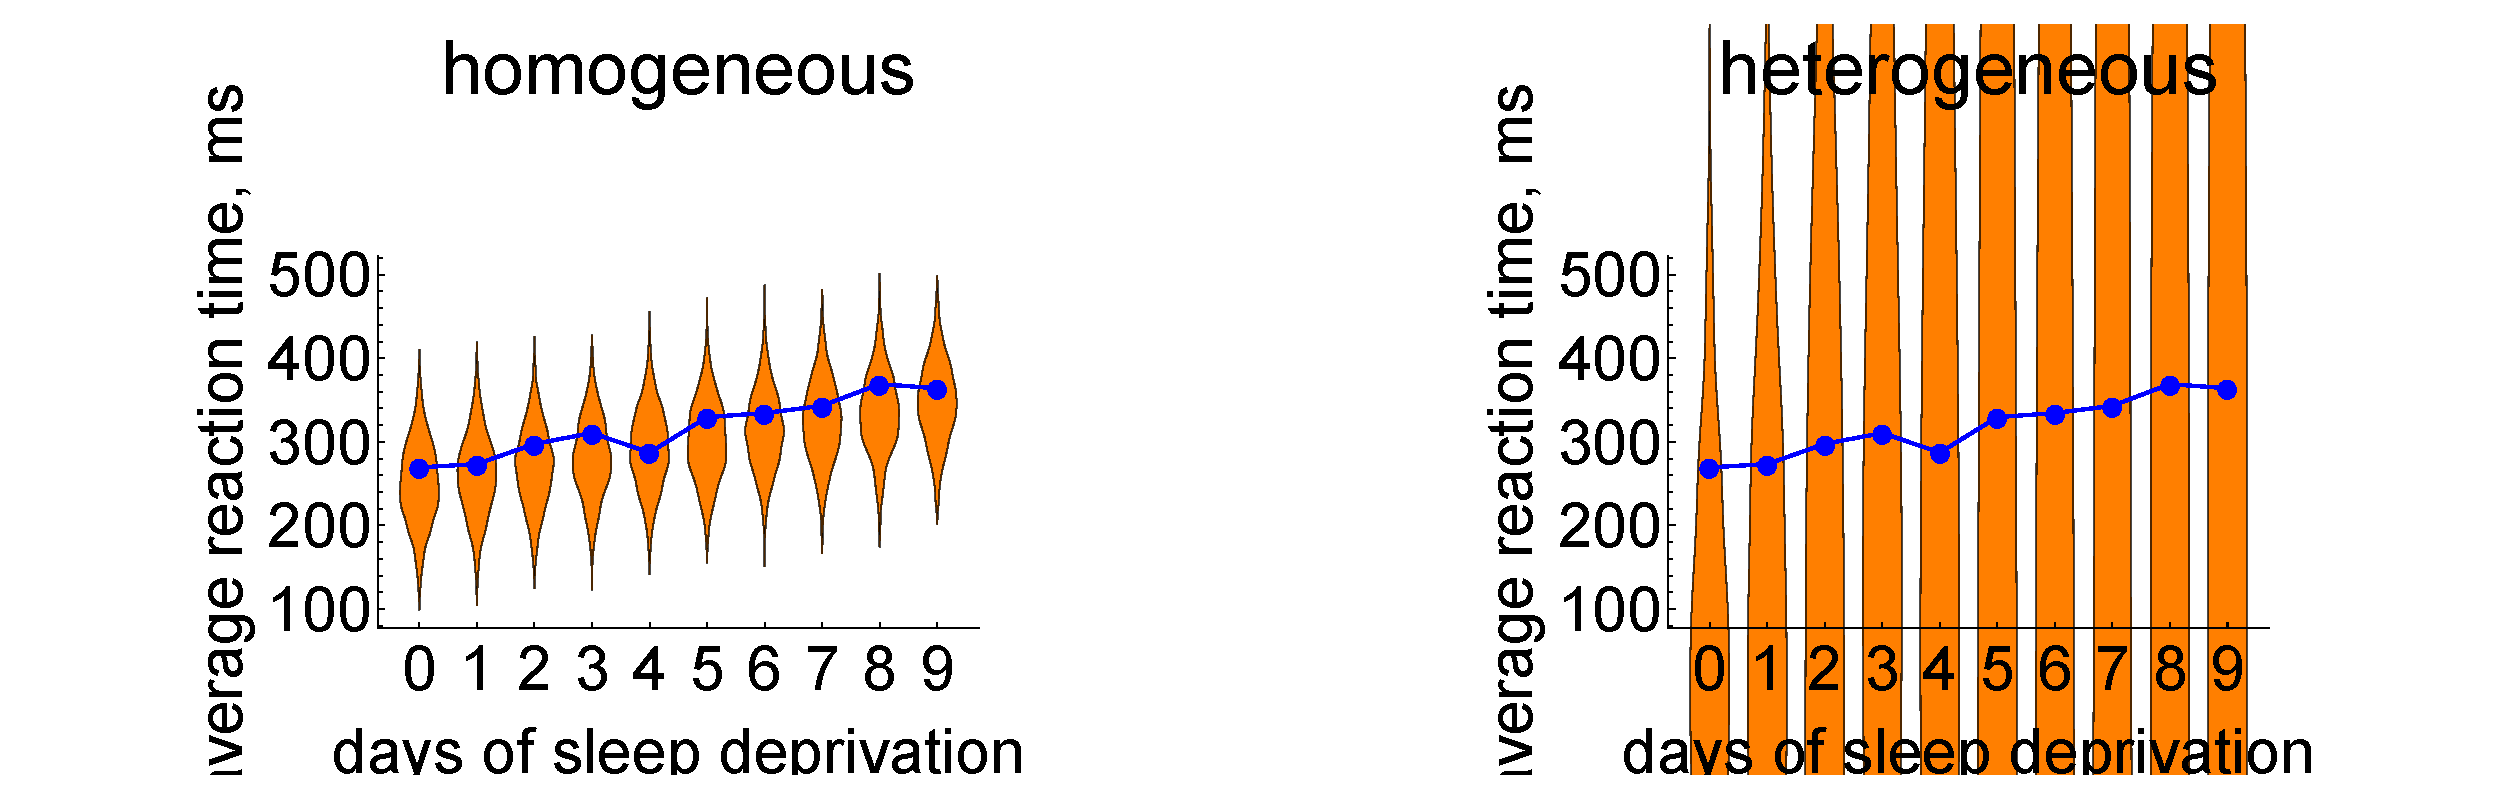
\includegraphics[width=1.5\textwidth]{figures/lec6_homoheteroTerrible.pdf}}
	\caption{The posterior predictive distribution (orange) and the data for subject 18 for a model fitted to the other 17 subjects' data, across the homogeneous coefficients (left), and heterogeneous coefficients (right) models.}\label{fig:lec6_homoheteroTerrible}
\end{figure}

\begin{problem}
	Alternatively we can fit a hierarchical model to the data which (hopefully) captures some of the best elements of each of the aforementioned models. Here we assume that the individual $(\alpha,\beta)$ for each subject are allowed to vary, but there is some overarching ``population-level'' distribution from which they are drawn. Assume that the coefficients have the following relationships:
	\begin{align}
	\alpha_i &\sim normal(a,b)\\
	\beta_i &\sim normal(c,d)\\
	a &\sim normal(100,100)\\
	b &\sim cauchy(0,5)\\
	c &\sim normal(10,5)\\
	d &\sim cauchy(0,1)
	\end{align}
	
	Code up the above model and compare the posterior distribution for $\beta$ for the hierarchical model, with those from the heterogeneous ones.
\end{problem}

The posterior distribution for the parameters exhibits shrinkage towards the grand mean (figure \ref{fig:lec6_sleepShrinkage}). In general those parameter estimates with a. the highest uncertainty, and b. lie furthest away from the mean, are shrunk the most in hierarchical models.

\begin{figure}[ht]
	\centerline{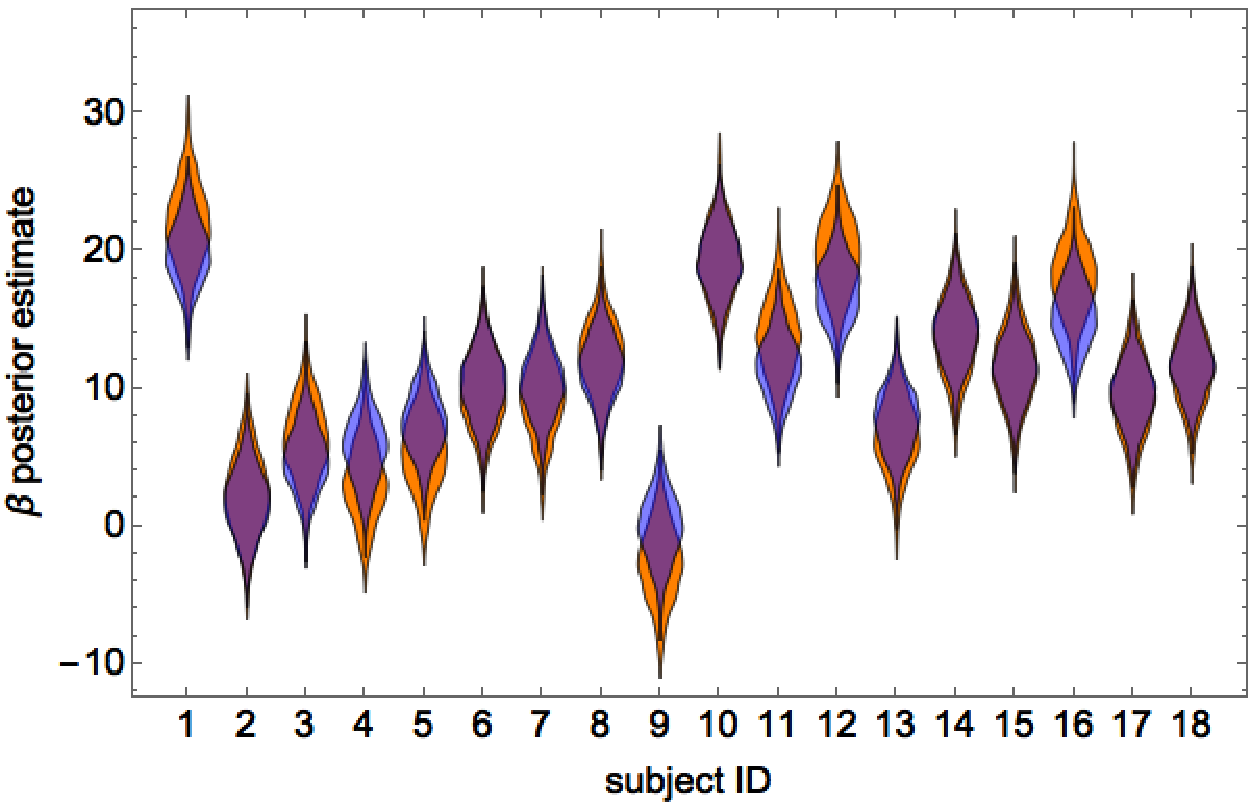
\includegraphics[width=1.5\textwidth]{figures/lec6_sleepShrinkage.pdf}}
	\caption{The posterior estimates of $\beta$ for the heterogeneous estimates (orange) versus the hierarchical estimates (blue).}\label{fig:lec6_sleepShrinkage}
\end{figure}

\begin{problem}
	Graph the posterior distribution for $\beta$ for another individual (not in the original dataset). How does this distribution compare to the value of $\beta$ obtained from the homogeneous coefficient model? (Hint: use the ``generated quantities'' block to generate samples of $\beta$ from the top-level parameters c and d.)
\end{problem}

The code to sample a value of $\beta$ for an out-of-sample individual is given below:
\begin{minted}{stan}
generated quantities {
  real aBeta;
  aBeta = normal_rng(c,d);
}
\end{minted}

The posterior distribution for $\beta$ has a mean of 10.2 (about the same as the original homogeneous estimate), but is wider (figure \ref{fig:lec6_sleepOverall}).

\begin{figure}[ht]
	\centerline{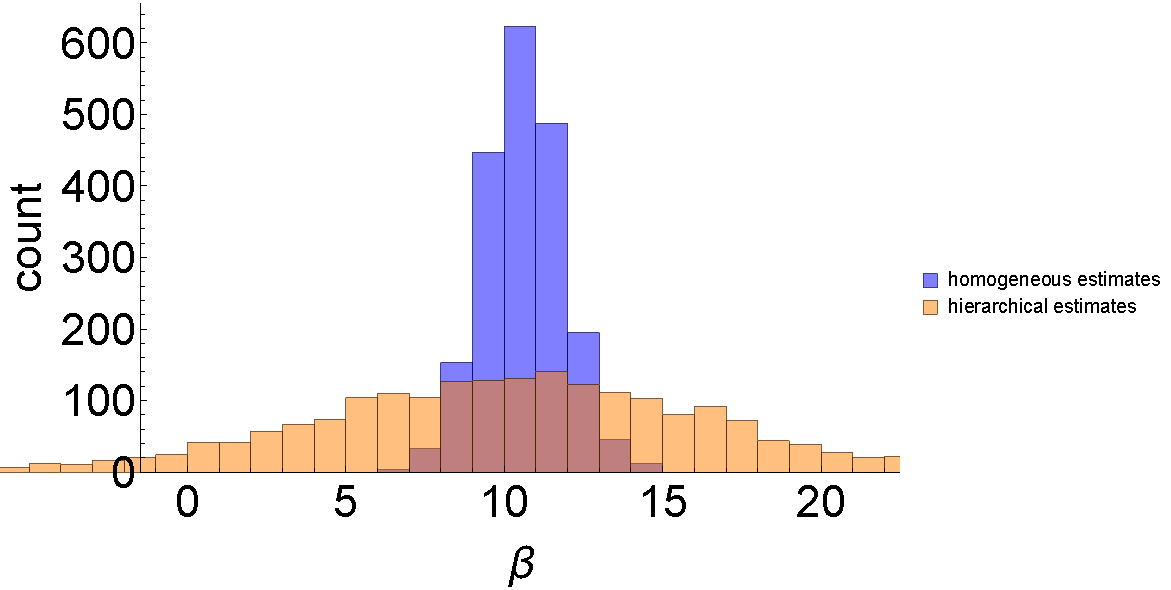
\includegraphics[width=1\textwidth]{figures/lec6_sleepHierarchicalBetaOverall.pdf}}
	\caption{The posterior estimates of $\beta$ for an out-of-sample individual for the homogeneous coefficients and hierarchical models.}\label{fig:lec6_sleepOverall}
\end{figure}

\section{Hierarchical ODEs: Bacterial cell population growth}
	The file ``prob6\_odeData.csv'' contains data for 5 replicates of an experiment in which bacterial cell population numbers were measured over time (as in the lectures). The following model for bacterial population size is proposed to explain the data:
	
\begin{equation}
\frac{\mathrm{d}N}{\mathrm{d}t} = \alpha N (1-\beta N)
\end{equation}

However measurement of bacterial cell numbers is subject to random, uncorrelated measurement error:

\begin{equation}
N^*(t) \sim \text{normal}(N(t), \sigma)
\end{equation}

where $N^*(t)$ is the measured number of cells, and $N(t)$ is the true population size. Finally we suppose that the initial number of bacteria cells is unknown, and hence must be estimated.

Further we assume the following priors:

\begin{align*}
\alpha&\sim normal(0,2)\\
\beta&\sim normal(0,2)\\
\sigma&\sim cauchy(0,1)\\
N(0) &\sim normal(5,2)
\end{align*}

where all parameters have a lower value of zero.
	
\begin{problem}
	Write a Stan function that returns $\frac{\mathrm{d}N}{\mathrm{d}t}$. (Hint 1: this will need to be done within the ``functions'' block at the top of the Stan file. Hint 2: the function must have a structure: 
\begin{minted}{stan}
    real[] bacteria_deriv(real t,real[] y,real[] theta,real[] x_r,int[] x_i)
\end{minted}
	where the variables $x_i$ and $x_r$ are not used here, but nonetheless need to be defined:
	
\begin{minted}{stan}
transformed data {
    real x_r[0];
    int x_i[0];
}
\end{minted}
)
	
\end{problem}

\begin{problem}
	Estimate a model where the parameters $(\alpha,\beta)$ are assumed to be the same across all experimental replicates.
\end{problem}

\begin{minted}{stan}
functions {
    real[] bacteria_deriv(real t,real[] y,real[] theta,real[] x_r,int[] x_i) {
    real dydt[1];
    
    dydt[1] = theta[1] * y[1] * (1 - theta[2] * y[1]);

    return dydt;
    }
}
data {
    int<lower=1> T;
    int<lower=0> N;
    real t0;
    real ts[T];
    matrix[T,N] y;
}
transformed data {
    real x_r[0];
    int x_i[0];
}
parameters {
      real<lower=0,upper=2> theta[2]; // Contains parameters (alpha,beta)
      real<lower=0> sigma;
      real<lower=0,upper=10> y0[1];
}
model {
    real y_hat[T,1];
    sigma ~ cauchy(0,1);
    theta ~ normal(0,2);
    y0 ~ normal(5,2);
    y_hat = integrate_ode(bacteria_deriv, y0, t0, ts, theta, x_r, x_i);
    for (i in 1:N){
        for (t in 1:T) {
            y[t,i] ~ normal(y_hat[t,1],sigma);
      }
  }
}

// Use this to capture the log-likelihood for later parts of the question
generated quantities {
    vector[N*T] logLikelihood;
    int k;
    real y_hat[T,1];
  
    k = 1;
    y_hat = integrate_ode(bacteria_deriv, y0, t0, ts, theta, x_r, x_i);
  
    for (i in 1:N){
       for (t in 1:T){
          logLikelihood[k] = normal_log(y[t,i],y_hat[t,1],sigma);
          k = k + 1;
       }
  }
}
\end{minted}

The posteriors for $(\alpha,\beta)$ are shown in figure \ref{fig:homogeneous_estimates}.

\begin{figure}[ht]
	\centerline{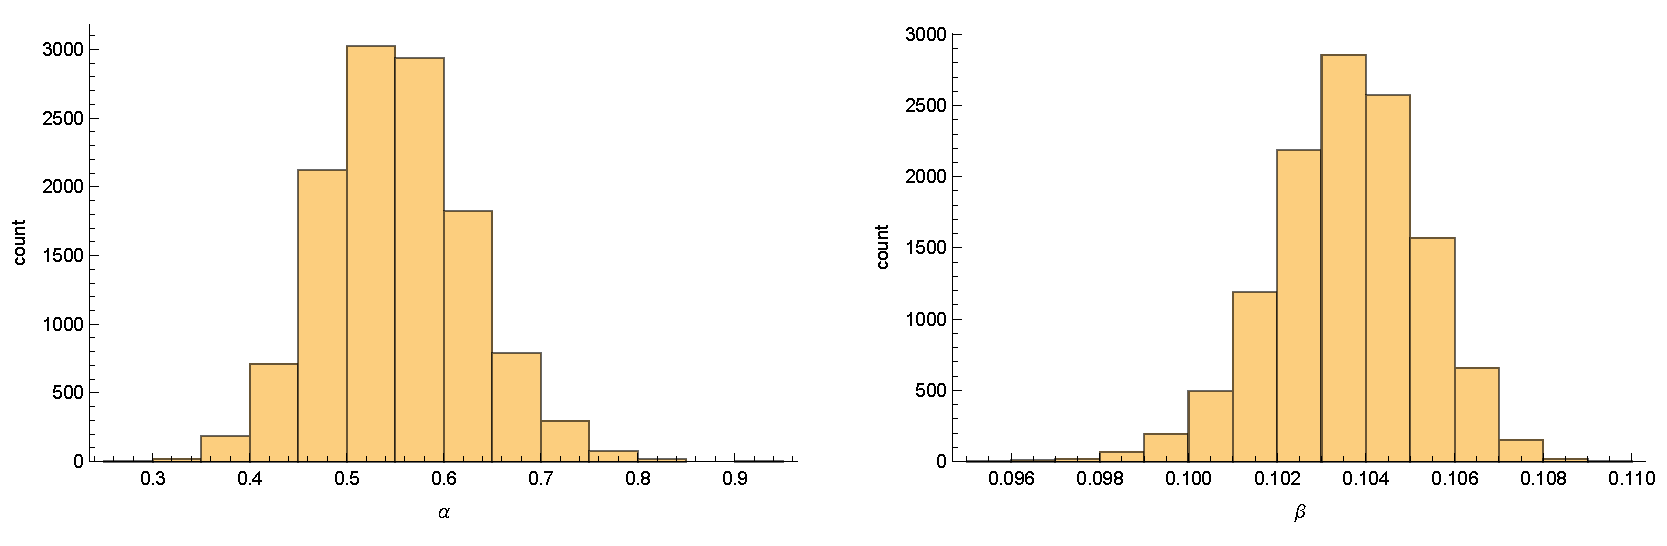
\includegraphics[width=1\textwidth]{figures/prob6_alphaBeta.pdf}}
	\caption{Homogeneous model estimates of $(\alpha,\beta)$.}\label{fig:homogeneous_estimates}
\end{figure}

\begin{problem}
	By graphing the data, or otherwise, comment on the assumption of a common $(\alpha,\beta)$ across all replicates.
\end{problem}

There is quite a clear variability between the replicates across different experiments (figure \ref{fig:time_series}). This makes the assumption of common parameter values across all replicates look quite weak. An alternative here would be to do some posterior predictive checks, but this isn't really needed here to be honest since the raw data plots are illuminating.

\begin{figure}[ht]
	\centerline{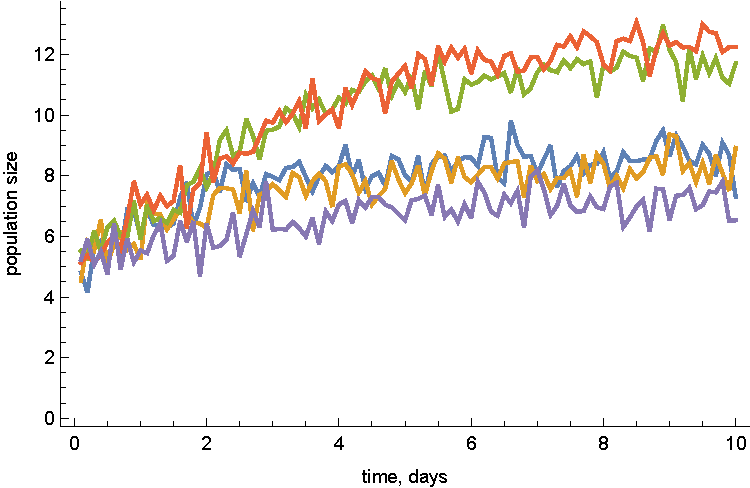
\includegraphics[width=1\textwidth]{figures/prob6_timeSeries.pdf}}
	\caption{Time series plot of 5 experimental replicates.}\label{fig:time_series}
\end{figure}


\begin{problem}
	Now estimate a model that estimates separate values for $(\alpha,\beta)$ across all replicates. Graph the posterior distribution for each parameter.
\end{problem}

\begin{minted}{stan}
parameters {
    real<lower=0,upper=2> theta[N,2];
    real<lower=0> sigma;
    real<lower=0,upper=10> y0[1];
}
model {
    real y_hat[T,1];
    sigma ~ cauchy(0,1);
    y0 ~ normal(5,2);
  
    for (i in 1:N){
        theta[i] ~ normal(0,2);
        y_hat = integrate_ode(bacteria_deriv, y0, t0, ts, theta[i], x_r, x_i);
        for (t in 1:T) {
             y[t,i] ~ normal(y_hat[t,1],sigma);
        }
   }
}

generated quantities {
    vector[N*T] logLikelihood;
    int k;
    real y_hat[T,1];
  
  k = 1;

    for (i in 1:N){
        y_hat = integrate_ode(bacteria_deriv, y0, t0, ts, theta[i], x_r, x_i);
        for (t in 1:T){
            logLikelihood[k] = normal_log(y[t,i],y_hat[t,1],sigma);
            k = k + 1;
        }
     }
}
\end{minted}


There is considerable heterogeneity in posterior estimates of $(\alpha,\beta)$ (figure \ref{fig:posterior_hetero})

\begin{figure}[ht]
	\centerline{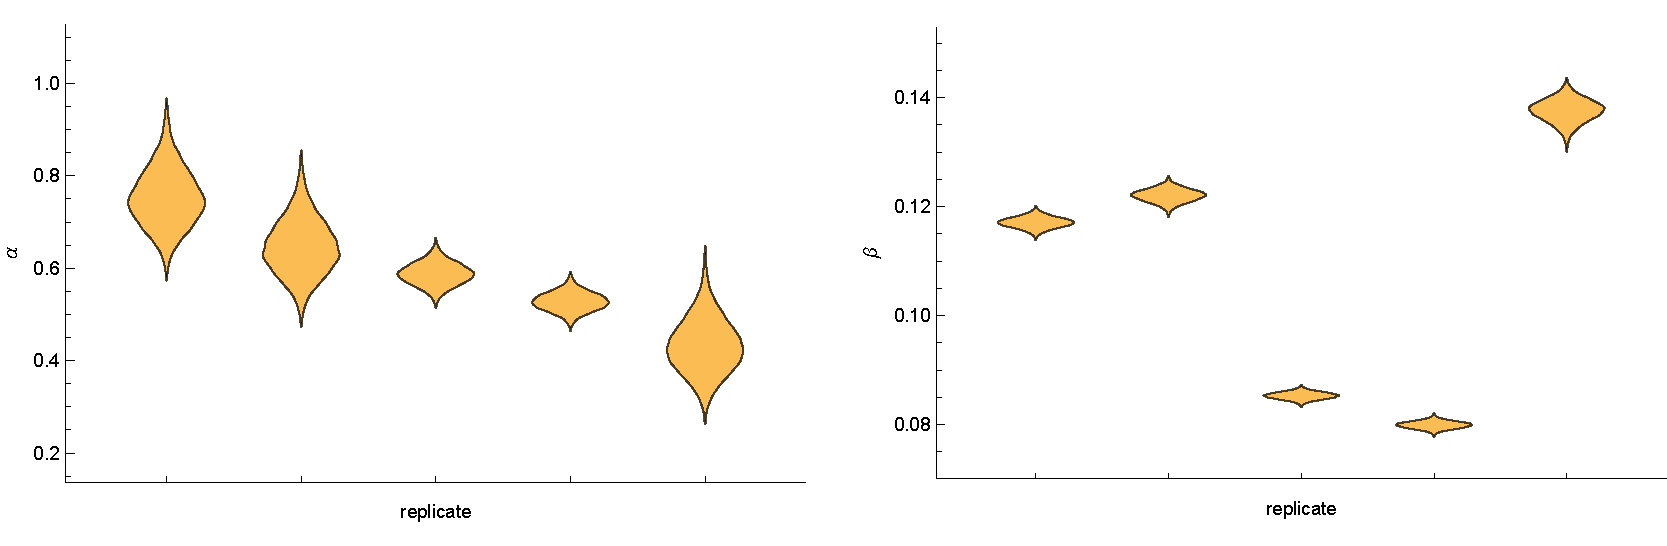
\includegraphics[width=1\textwidth]{figures/prob6_heteroAlphaBeta.pdf}}
	\caption{Posterior parameter estimates for heterogeneous model.}\label{fig:posterior_hetero}
\end{figure}

\begin{figure}[ht]
	\centerline{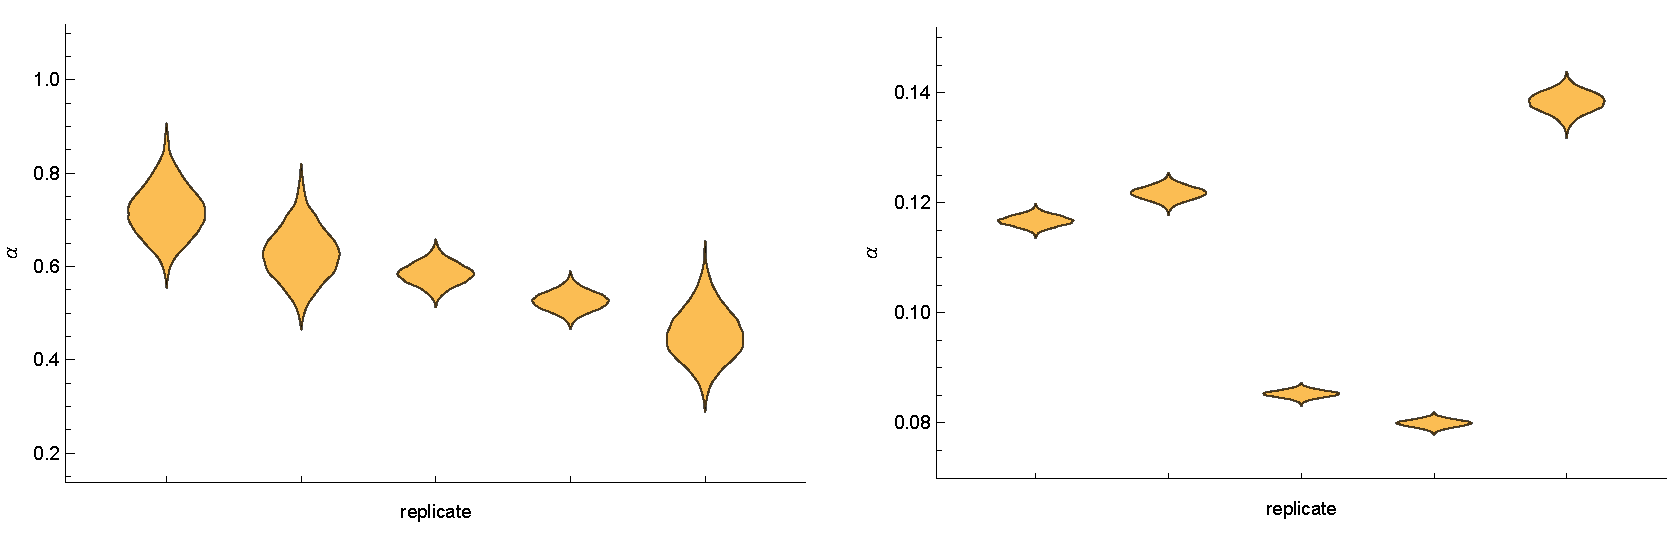
\includegraphics[width=1\textwidth]{figures/prob6_hierAlphaBeta.pdf}}
	\caption{Posterior parameter estimates for hierarchical model.}\label{fig:posterior_hier}
\end{figure}

\begin{problem}
	Estimate a hierarchical model assuming the following priors:
	
	\begin{align*}
	\alpha&\sim gamma(a,b)\\
	\beta&\sim gamma(c,d)\\
	a&\sim normal(20,5)\\
	b&\sim normal(40,5)\\
	c&\sim normal(10,3)\\
	d&\sim normal(100,5)
	\end{align*}
	
	Compare your estimates of $(\alpha,\beta)$ with those from the completely heterogeneous model.
\end{problem}

\begin{minted}{stan}
functions {
    real[] bacteria_deriv(real t,real[] y,real[] theta,real[] x_r,int[] x_i) {
    real dydt[1];

    dydt[1] = theta[1] * y[1] * (1 - theta[2] * y[1]);

    return dydt;
    }
}
data {
    int<lower=1> T;
    int<lower=0> N;
    real t0;
    real ts[T];
    matrix[T,N] y;
}
transformed data {
    real x_r[0];
    int x_i[0];
}
parameters {
    real<lower=0> a1[2];
    real<lower=0> a2[2];
    real<lower=0,upper=2> theta[N,2];
    real<lower=0> sigma;
    real<lower=0,upper=10> y0[1];
}
model {
    real y_hat[T,1];
    a1[1] ~ normal(20,5);
    a1[2] ~ normal(40,5);
    a2[1] ~ normal(10,3);
    a2[2] ~ normal(100,5);

    sigma ~ cauchy(0,1);
    y0 ~ normal(5,2);

    for (i in 1:N){
        theta[i,1] ~ gamma(a1[1],a1[2]);
        theta[i,2] ~ gamma(a2[1],a2[2]);
        y_hat = integrate_ode(bacteria_deriv, y0, t0, ts, theta[i], x_r, x_i);
        for (t in 1:T) {
            y[t,i] ~ normal(y_hat[t,1],sigma);
        }
     }
}

generated quantities {
    vector[N*T] logLikelihood;
    int k;
    real y_hat[T,1];
    real aTheta[2];
    real y_hat_overall[T,1];

    aTheta[1] = gamma_rng(a1[1],a1[2]);
    aTheta[2] = gamma_rng(a2[1],a2[2]);
    y_hat_overall = integrate_ode(bacteria_deriv, y0, t0, ts, aTheta, x_r, x_i);

    k = 1;

    for (i in 1:N){
        y_hat = integrate_ode(bacteria_deriv, y0, t0, ts, theta[i], x_r, x_i);
        for (t in 1:T){
            logLikelihood[k] = normal_log(y[t,i],y_hat[t,1],sigma);
            k = k + 1;
        }
    }
}
\end{minted}

There is very limited shrinkage versus the purely heterogeneous model (figure \ref{fig:posterior_hetero} versus figure \ref{fig:posterior_hier}.) This is because there is quite a lot of data for each replicate.

\begin{problem}
	Estimate the overall $(\alpha,\beta)$ for the hierarchical model. How do these compare to the pooled model estimates?
\end{problem}

The estimates reflect greater uncertainty compared to the pooled model (figure \ref{fig:posterior_hierOverall} versus figure \ref{fig:homogeneous_estimates}). This is desirable since the pooled model understates uncertainty.

\begin{figure}[ht]
	\centerline{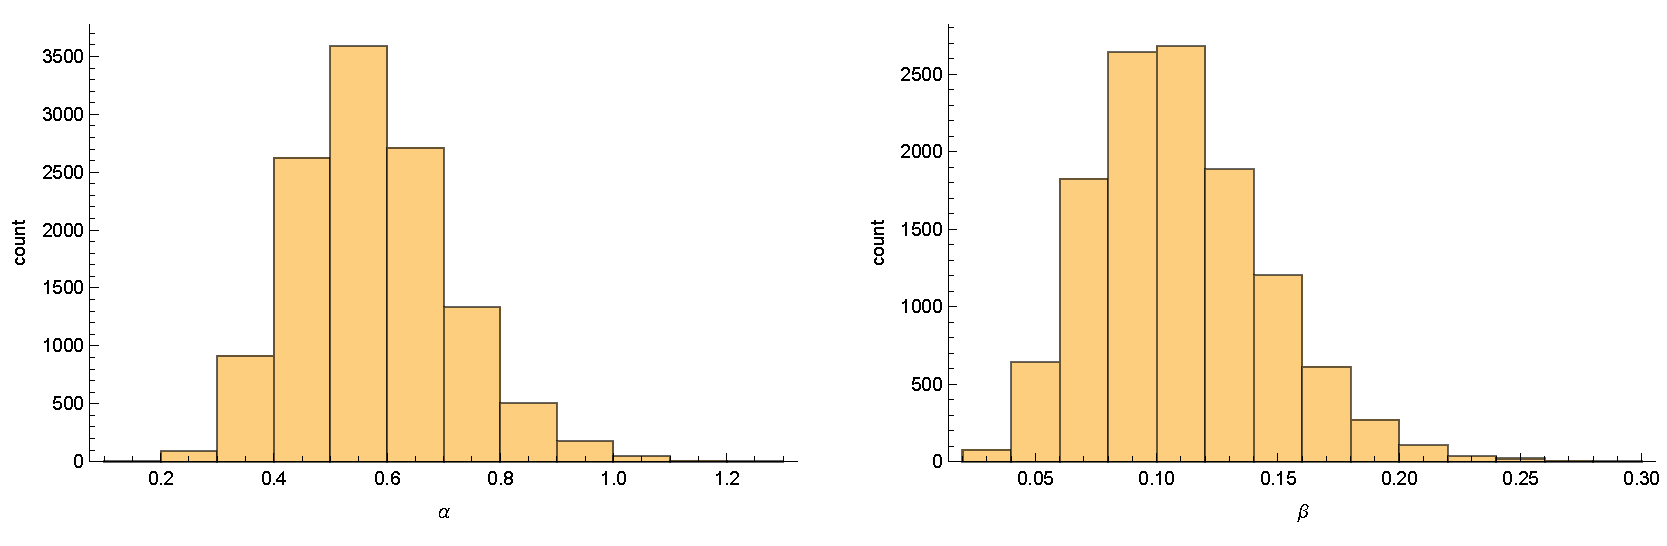
\includegraphics[width=1\textwidth]{figures/prob6_overallAlphaBeta.pdf}}
		\caption{Overall parameter estimates for the posterior parameters in the hierarchical model.}\label{fig:posterior_hierOverall}
	\end{figure}


\begin{problem}
	By holding out one of your datasets, compare the predictive performance of each model.
\end{problem}

I haven't done this yet, but it will certainly favour the hierarchical model (the pooled model performs considerably worse using naive estimates of model performance.)

\section{Bowel cancer model selection}
The file ``prob6\_cancer.csv'' contains (fictitious) data on the population size of a given county ($N$) and the number of bowel cancer cases in that county ($X$). In this question we aim to build a model to estimate the underlying rate of cancer occurrence $\lambda$.

\begin{problem}
	A simple model is to assume that cancer occurrence is an independent event, and hence we use the following model,
	\begin{equation}
	 X_i \sim \text{poisson}(N_i\lambda)
	\end{equation}
	where $N_i$ is the population in county $i$, and $X_i$ is the number of cases of bowel cancer in the same county. In Stan write a model to estimate the underlying rate of bowel cancer occurrence ($\lambda$), where we assume a prior of the form $\lambda\sim \text{normal}(0.5,0.5)$.
\end{problem}

\begin{minted}{Stan}
data{
  int K;
  vector[K] N;
  int X[K];
}
parameters{
  real<lower=0> lambda;
}
model{
  X ~ poisson(lambda*N);
  lambda ~ normal(0.5,0.5);
}
\end{minted}

which should estimate $\lambda\approx 0.1$.

\begin{problem}
	Using the \mintinline{Stan}{generated quantities} section record the estimated log likelihood of each data point, for each posterior sample of $\lambda$.
\end{problem}

\begin{minted}{Stan}
generated quantities{
  vector[K] lLoglikelihood;
  for(i in 1:K)
    lLoglikelihood[i] = poisson_lpmf(X[i]|N[i]*lambda);
}
\end{minted}

\begin{problem}
	By using Stan's \mintinline{Stan}{optimizing} function to obtain the MAP estimate of $\lambda$, estimate the expected log pointwise predictive density (elpd) via a DIC method,
	\begin{equation}
	\widehat{\text{elpd}} = log \;p(X|\hat{\theta}_{Bayes}) - \underbrace{2 V_{s=1}^{S}log\; p (X|\theta_s)}_{DIC}
	\end{equation}
	where $V_{s=1}^{S} log\; p (X|\theta_s)$ is the variance in log-likelihood for all data points across $S$ posterior draws. Hint: the latter part of the formula requires that we estimate the model by sampling.
\end{problem}

The MAP estimates of the model log-likelihood can be determined using,

\begin{minted}{R}
bFit <- optimizing(aModel,data=list(X=X,N=N,K=length(N)))
likelihoodBayes <- sum(bFit$par[2:1001])
\end{minted}

Then estimating the model by sampling we can then obtain the $p_{DIC}$ term,

\begin{minted}{R}
fit <- sampling(aModel,data=list(X=X,N=N,K=length(N)),iter=200,chains=4)
lLoglikelihood <- extract_log_lik(fit,'lLoglikelihood')
aLogLikelihood <- rowSums(lLoglikelihood)
pDIC <- 2 * var(aLogLikelihood)
\end{minted}

which we then use to estimate $\widehat{\text{elpd}}$,

\begin{minted}{R}
aDIC <- likelihoodBayes - pDIC
\end{minted}

which should be $\approx$ -3996.

\begin{problem}
	Estimate $\text{elpd}$ using the AIC method. Hint: use Stan's \mintinline{Stan}{optimizing} function where the Stan file has had the prior commented out, to achieve the maximum likelihood estimate of the log-likelihood.
\end{problem}

The AIC method penalises the estimated log-likelihood by one since there is only a single parameter in the model. Hence this estimate can be obtained by using,

\begin{minted}{R}
bModel <- stan_model('poissonCancerML.stan')
bFit <- optimizing(bModel,data=list(X=X,N=N,K=length(N)))
likelihoodML <- sum(bFit$par[2:1001])
aAIC <- likelihoodML - 1
\end{minted}

which should yield $\approx$ -3996 (it's slightly higher than that obtained from the DIC method).



\begin{problem}
	Either manually or using the ``loo'' package in R estimate the elpd by a WAIC method. If you choose the manual method, this can be done with the following formula,
	
	\begin{equation}
	\widehat{\text{elpd}}  = \underbrace{\sum_{i=1}^{N} log\left(\frac{1}{S}\sum_{s=1}^{S} p(X_i|\theta_s)\right)}_{\text{log pointwise predictive density}} - p_{WAIC}
	\end{equation}
	
	where $p_{WAIC} =  \sum_{i=1}^{N}V_{s=1}^{S} var_{post} \left[log\; p(X_i|\theta_s)\right]$.
\end{problem}

Using the loo package this is quite straightforward,

\begin{minted}{R}
library(loo)
lLoglikelihood <- extract_log_lik(fit,'lLoglikelihood')
aWAIC <- waic(lLoglikelihood)
\end{minted}

which should yield a value of $\approx$ -3999 with a standard error that I think is wrong (sad, sad face).

Alternatively, doing this manually,

\begin{minted}{R}
library(matrixStats)
bWAIC_1 <- sum(sapply(seq(1,1000,1),function(i) logSumExp(lLoglikelihood[,i])-log(400)))
bWAIC_p <- sum(sapply(seq(1,1000,1), function(i) var(lLoglikelihood[,i])))
bWAIC <- bWAIC_1 - bWAIC_p
\end{minted}

where I have used \mintinline{R}{logSumExp} because it is more numerically stable than doing the piecewise application of the exponential. This should yield a value identical to that obtained via loo $\approx$ -3999.

\begin{problem}
	By partitioning the data into 10 folds of training and testing sets (where one data point occurs in each testing set once only), estimate the out-of-sample predictive capability of the model. Hint 1: in R use the ``Caret'' package's \mintinline{R}{createFolds} to create 10 non-overlapping folds. Hint 2: adjust your Stan program to calculate the log-likelihood on the test set.
\end{problem}

In R the folds can be created by,

\begin{minted}{R}
lFolds <- createFolds(X)
\end{minted}

The Stan program can be changed to the below which allows the estimation of out-of-sample predictive capability using,

\begin{minted}{Stan}
data{
  int KTrain;
  vector[KTrain] NTrain;
  int XTrain[KTrain];
  # Hold out set
  int KTest;
  vector[KTest] NTest;
  int XTest[KTest];
}
parameters{
  real<lower=0> lambda;
}
model{
  XTrain ~ poisson(lambda*NTrain);
  lambda ~ normal(0.5,0.5);
}
generated quantities{
  vector[KTest] lLoglikelihood;
  for(i in 1:KTest)
    lLoglikelihood[i] = poisson_lpmf(XTest[i]|NTest[i]*lambda);
}
\end{minted}

Then we create a loop in R that stores the log-likelihood for each fold,

\begin{minted}{R}
vLogLikelihood <- vector(length=10,mode = 'list')
for(i in 1:10){
  print(i)
  aFold <- lFolds[[i]]
  XTrain <- X[-aFold]
  NTrain <- N[-aFold]
  XTest <- X[aFold]
  NTest <- N[aFold]
  aFit <- sampling(aModel,data=list(XTrain=XTrain,NTrain=NTrain,KTrain=length(NTrain),
                          XTest=XTest,NTest=NTest,KTest=length(NTest)),iter=200,chains=4)
  vLogLikelihood[[i]] <- extract_log_lik(aFit,'lLoglikelihood')
}
\end{minted}

From which we can estimate the elpd by,

\begin{minted}{R}
aLogTotal <- 0
for(i in 1:10){
  aLogLikeTemp <- vLogLikelihood[[i]] 
  aLogTotal <- aLogTotal + sum(colMeans(aLogLikeTemp))
}
\end{minted}

which should yield $\approx$ -3997. So in this case all measures look reasonably close to the value obtained by cross-validation.

\begin{problem}
	A colleague suggests fitting a negative binomial sampling model to the data, in case over-dispersion exists. Using a prior $\kappa\sim \text{log-normal}(0,0.5)$ on the dispersion parameter, change your Stan model to use this distribution, and estimate the out-of-sample predictive density using any of the previous methods. Which model do you prefer? Hint: use Stan's \mintinline{Stan}{neg_binomial_2} function to increment the log-probability.
\end{problem} 

The new Stan program should look something like,

\begin{minted}{Stan}
data{
  int KTrain;
  vector[KTrain] NTrain;
  int XTrain[KTrain];
  # Hold out set
  int KTest;
  vector[KTest] NTest;
  int XTest[KTest];
}
parameters{
  real<lower=0> lambda;
  real<lower=0> kappa;
}
model{
  XTrain ~ neg_binomial_2(lambda*NTrain,kappa);
  lambda ~ normal(0.5,0.5);
  kappa ~ lognormal(0,0.5);
}
generated quantities{
  vector[KTest] lLoglikelihood;
  for(i in 1:KTest)
    lLoglikelihood[i] = neg_binomial_2_lpmf(XTest[i]|NTest[i]*lambda,kappa);
}
\end{minted}

And via manual cross-validation (the best method available here) I obtain an estimated elpd $\approx$ -2731. So the negative binomial model is a significantly better fit to the data on the face of it. However, to do this comparison correctly it is necessary to do pairwise comparison, which takes the variability in log likelihood into account, then compares a $z$ score with a standard normal,

\begin{minted}{R}
z <- sum(lLoglikelihood1-lLoglikelihood2)
        /(sqrt(length(lLoglikelihood1))*sd(lLoglikelihood1-lLoglikelihood2))
p <- 1 - pnorml(z)
\end{minted}

which will be tiny here.

\begin{problem}
	A straightforward way to estimate the marginal likelihood is to use,
	
	\begin{equation}
	p(X) \approx \frac{1}{S} \sum_{s=1}^S p(X|\theta_s)
	\end{equation}
	
	where $\theta_s\sim p(\theta)$. Either using Stan's \mintinline{Stan}{generated quantities} block or otherwise estimate the marginal likelihood of the poisson model. Hint: if you use Stan then you need to use \mintinline{R}{log_sum_exp} to marginalise the sampled log probabilities.
\end{problem}

In Stan this can be done using the following block,

\begin{minted}{Stan}
generated quantities{
   real loglikelihood;
   real<lower=0> lambda1;
   lambda1 = normal_rng(0.5,0.5);
   while(lambda1 <= 0)
     lambda1 = normal_rng(0.5,0.5);
   loglikelihood = 0;
   for(i in 1:K)
     loglikelihood = loglikelihood + poisson_lpmf(X[i]|lambda1*N[i]);
}
\end{minted}

Note in the above we are using samples from the prior \textbf{not} the posterior. The above is just using Stan like a random number generator. We can then estimate the marginal likelihood by doing the following in R,

\begin{minted}{R}
library(matrixStats)
lMarginalLog <- extract(fit,'loglikelihood')[[1]]
logSumExp(lMarginalLog)
\end{minted}

which should yield a value $\approx$ -3991. However there is a large variance in this estimator for more complex models.

\begin{problem}
	Estimate the marginal likelihood of the negative binomial model, and hence estimate the log Bayes Factor. Which model do you prefer?
\end{problem}

This is best computed on the log scale (using the output from logSumExp), and should yield something like $\text{log}\;BF\approx 1200$ in favour of the negative binomial model. 

\bibliographystyle{plain} 
\bibliography{Bayes}

\end{document}
